\scanpage{87}
% manuscript lines 1–2
\deleted{\uline{\unsure{Déf.|Prop.}}} \uline{Lemme} Soient $A$ un anneau, $B$ une algèbre finie sur $A$, $M$ un $B$-mod de type fini.

% manuscript lines 3
(i) Si $M_{[A]}$ est $(S_k)$, il en est de $=$ de $M$

% manuscript lines 4–6
(ii) Supposons que pour \deleted{\unsure{tt}} idéaux premiers $\mathfrak q,\mathfrak q'$ de $B$, induisant \inserted{le $=$} $\mathfrak p$ sur $A$, on ait $\dim M_{\mathfrak q}=\dim M_{\mathfrak q'}$. Alors si $M$ est $(S_k)$ sur $B$, il est $(S_k)$ sur $A$.

% manuscript lines 7
On peut supposer $A\subset B$, \deleted{$\operatorname{Spec}\unsure{A|B}$} $\operatorname{Supp} M=\operatorname{Sp} B$

% manuscript lines 8–11
\uline{Dém} (i) Soit $\deleted{\unsure{\mathfrak p|\mathfrak q}}\mathfrak q\in\operatorname{Sp} A$, \deleted{si $\dim M_{\mathfrak p}\leq k$ \unsure{induisant} $\mathfrak q$ sur $A$, l'hypothèse indique que $\dim_{A_{\mathfrak q}}M_{\mathfrak q}=\dim_{B_{\mathfrak p}} M_{\mathfrak p}$, or \unsure{d'ailleurs} \unsure{par hypothèse}, on a $\operatorname{prof}$ [a fortiori $\dim_{A_{\mathfrak q}}M_{\mathfrak q}\geq\operatorname{Sup}_{\mathfrak p\,\mathrm{sur}\,\mathfrak q}\dim_{B_{\mathfrak p}}M_{\mathfrak p}$] et} on a

% manuscript lines 12
\[
\deleted{\text{si}}\quad \operatorname{prof}_{A_{\mathfrak q}} M_{\mathfrak q}=\mathop{\mathrm{Inf}}_{\mathfrak p\,\mathrm{sur}\,\mathfrak q}\operatorname{prof}_{B_{\mathfrak p}}M_{\mathfrak p},\quad
\deleted{\text{donc}}\quad \dim_{A_{\mathfrak q}}M_{\mathfrak q}=\mathop{\mathrm{Sup}}_{\mathfrak p\,\mathrm{sur}\,\mathfrak q}\dim_{B_{\mathfrak p}}M_{\mathfrak p}
\]

% manuscript lines 13
donc si $\mathfrak p$ sur $\mathfrak q$
\[
\operatorname{prof}_{B_{\mathfrak p}}M_{\mathfrak p}\geq\operatorname{prof}_{A_{\mathfrak q}}M_{\mathfrak q}\geq\operatorname{Inf}(k,\dim_{A_{\mathfrak q}}M_{\mathfrak q})\geq\operatorname{Inf}(k,\dim_{B_{\mathfrak p}}M_{\mathfrak p}),\quad\text{ck.}
\]

% manuscript lines 14–17
(ii) On a ici, grâce à l'hyp. spéciale
\[
\dim_{A_{\mathfrak q}}M_{\mathfrak q}=\dim_{A_{\mathfrak p}}M_{\mathfrak p}
\]
Or pour $\mathfrak p$ \uline{convenable} sur $\mathfrak q$, on aura \deleted{d'où \unsure{$M$} \unsure{si} \illegible{3} \unsure{l'occasion},}
\[
\deleted{\operatorname{prof}_{A_{\mathfrak q}}M_{\mathfrak q}\geq}\quad \operatorname{prof}_{A_{\mathfrak q}}M_{\mathfrak q}=\operatorname{prof}_{B_{\mathfrak p}}M_{\mathfrak p}\quad(\text{i.e. on a }{\geq})
\]

% manuscript lines 18–21
\deleted{Pour les \unsure{vérif.}, pour un système d'hyp\unsure{.} \unsure{sous} \illegible{2} et \unsure{chacun} de $\unsure{k\geq A_{\mathfrak q}|M_{\mathfrak q}}$, \unsure{en sorte, on est amené à} \unsure{trouver} qu'\unsure{elle} est aussi vérifiée pour} d'où le résultat voulu \textendash\ \textendash\ \textendash\ \textendash

% manuscript lines 22
$\deleted{\mathfrak p\subset\mathfrak q}$

% manuscript lines 22–23
\diagram{\begin{tikzcd}[ampersand replacement=\&,row sep=small,column sep=small]
\deleted{B}\&\deleted{M}\\
\deleted{A}\arrow[u,dash]\&\deleted{\unsure{\mathfrak p}}
\end{tikzcd}}

% manuscript lines 24
$\operatorname{prof}\geq\operatorname{Inf}(k,\dim)$

% manuscript lines 4–23
% margin note written sideways
\margin{$\unsure{\pi_1(Y)}\longrightarrow\unsure{\pi_1(X)}$ \unsure{$\psi$ bijective} \unsure{$x\in X$} $\unsure{\geq2}$ $\unsure{\geq3}$ \unsure{depth} $\unsure{\geq2}\Rightarrow\psi$ surj \unsure{depth} $\unsure{\geq3}$, \unsure{conditions} \illegible{2} $\Rightarrow\psi$ bij}

% manuscript lines 24
\figure{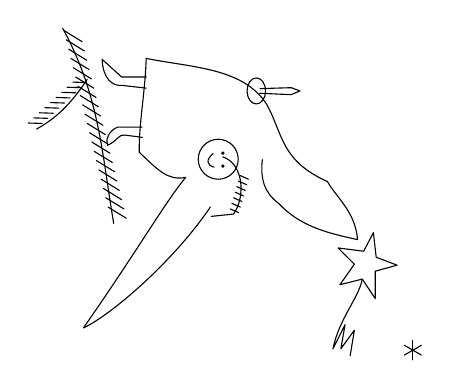
\begin{tikzpicture}[scale=.59,line cap=round,line join=round]
\begin{scope}[rotate=-90]
\draw (-2,0) .. controls (-1.8,1) and (-1.8,2.1) .. (-1,2.6) .. controls (-.35,2.95) and (.2,2.9) .. (.65,3.9) .. controls (1,4.1) and (1.3,4.5) .. (1.9,4.55) .. controls (1.75,3.85) and (1.6,3.3) .. (1.12,2.85) .. controls (.9,2.55) and (.6,2.45) .. (.18,2.5);
\draw (-2,0) .. controls (-1.2,-.03) and (-.6,-.16) .. (.02,-.15) .. controls (.4,.25) and (.64,.47) .. (.56,.85) .. controls (1.15,.37) and (2,-.1) .. (3.8,-1.35) .. controls (3.55,-.8) and (2.42,.55) .. (1.2,1.38);
\draw (-1.6,0)--(-1.6,-.53) .. controls (-1.8,-.75) and (-1.92,-.88) .. (-1.98,-.95) .. controls (-1.55,-.93) and (-1.4,-.72) .. (-1.42,-.52)--(-1.36,0);
\draw (-.52,-.09)--(-.52,-.62) .. controls (-.43,-.82) and (-.24,-.88) .. (-.13,-.83) .. controls (-.24,-.6) and (-.37,-.6) .. (-.35,-.46)--(-.3,-.08);
\draw (.12,1.65) .. controls (.27,2.1) and (.98,2.14) .. (1.35,1.88)--(1.4,1.4);
\draw (.17,1.55) circle (.43); \fill (.04,1.65) circle (.04) (.32,1.65) circle (.04); \draw (.05,1.44) .. controls (.18,1.28) and (.3,1.3) .. (.34,1.46);
\foreach \x in {0,...,6}{\draw (.52+.12*\x,2.02-.035*\x)--(.6+.12*\x,2.2-.035*\x);}
\draw (-1.3,2.37) ellipse (.28 and .2); \draw (-1.35,2.45)--(-1.37,3.12)--(-1.3,3.31)--(-1.22,3.12)--(-1.25,2.44);
\draw (2.45,5.4)--(2.58,4.93)--(3.17,4.93)--(2.75,4.65)--(2.87,4.17)--(2.43,4.48)--(2.08,4.13)--(2.15,4.68)--(1.75,4.89)--(2.28,4.95)--cycle;
\draw (2.75,4.65)..controls(3.15,4.58)and(3.6,4.15)..(4.25,4.02)--(3.73,4.28)--(4.25,4.19)--(3.85,4.48)--(4.4,4.39);
\foreach \a in {0,60,120}{\draw[shift={(4.28,5.74)},rotate=\a](-.21,0)--(.21,0);}
\draw (-2.65,-1.8)..controls(-1.2,-1)and(.1,-.95)..(1.55,-.7); \draw (-1.55,-1.27)..controls(-1.05,-1.6)and(-.72,-1.92)..(-.48,-2.36);
\foreach \i in {0,...,19}{\draw (-2.6+.2*\i,-1.77+.05*\i)--(-2.36+.2*\i,-1.38+.05*\i);}\foreach \i in {0,...,8}{\draw (-1.48+.11*\i,-1.28-.12*\i)--(-1.49+.11*\i,-1.58-.12*\i);}
\end{scope}\end{tikzpicture}}
% crop-candidate: scan 87
% archive sheet number: 86

